 % ****** Start of file main.tex ******

\documentclass[%
reprint,
amsmath,
amssymb,
aip,
rsi, 
numerical,
floatfix,
]{revtex4-1}

\usepackage{graphicx}% Include figure files
\usepackage{dcolumn}% Align table columns on decimal point
\usepackage{gensymb}
\usepackage[utf8]{inputenc}
\usepackage{xr}
\usepackage[dvipsnames]{xcolor}%Make nice color
\usepackage{siunitx}
\usepackage{upgreek}
\usepackage{bm}% bold math
%\usepackage{hyperref}% add hypertext capabilities
\usepackage[mathlines]{lineno}% Enable numbering of text and display math
%linenumbers\relax % Commence numbering lines

%% OWN Commands
\newcommand{\myCite}[1]{\textcolor{blue}{\cite{#1}}}
\newcommand{\myOnlineCite}[1]{\textcolor{blue}{\onlinecite{#1}}}
\begin{document}

\title{\textcolor{blue}{Calibration of the absolute light--yield of various scintillator screens for electron bunch charge determination in laser--plasma accelerators}}

\author{\firstname{Thomas} Kurz}
\email[E-Mail adress: ]{t.kurz@hzdr.de}
 \affiliation{Helmholtz--Zentrum Dresden--Rossendorf, Bautzner Landstraße 400,D-01328 Dresden, Germany}
 \affiliation{Ludwig--Maximilians--Universität München, Am Coulombwall 1, D-85748 Garching, Germany}
 \affiliation{Technische Universität Dresden, D-01069 Dresden, Germany}
 
\author{\surname{Jakob Matthias} Krämer}
 \affiliation{Helmholtz--Zentrum Dresden--Rossendorf, Bautzner Landstraße 400,D-01328 Dresden, Germany}
 \affiliation{Technische Universität Dresden, D-01069 Dresden, Germany}
 
\author{\surname{Jurjen Pieter} Couperus}
 \affiliation{Helmholtz--Zentrum Dresden--Rossendorf, Bautzner Landstraße 400,D-01328 Dresden, Germany}
 \affiliation{Technische Universität Dresden, D-01069 Dresden, Germany}
 
\author{\firstname{Hao} Ding}
 \affiliation{Ludwig--Maximilians--Universität München, Am Coulombwall 1, D-85748 Garching, Germany}
 \affiliation{Max--Planck--Institut für Quantenoptik, Hans-Kopfermann-Straße 1, D-85748 Garching, Germany}
 
\author{\firstname{Stefan} Kuschel}
 \affiliation{Helmholtz--Institut Jena, Fröbelstieg 3, D-07743 Jena, Germany}
 \affiliation{Friedrich--Schiller--Universität Jena, Fürstengraben 1, D-07743 Jena, Germany}
 
\author{\surname{Alexander} Köhler}
 \affiliation{Helmholtz--Zentrum Dresden--Rossendorf, Bautzner Landstraße 400,D-01328 Dresden, Germany}
 \affiliation{Technische Universität Dresden, D-01069 Dresden, Germany} 
 
\author{\surname{Omid} Zarini}
 \affiliation{Helmholtz--Zentrum Dresden--Rossendorf, Bautzner Landstraße 400,D-01328 Dresden, Germany}
 \affiliation{Technische Universität Dresden, D-01069 Dresden, Germany}
 
\author{\firstname{Dominik} Hollatz}
 \affiliation{Helmholtz--Institut Jena, Fröbelstieg 3, D-07743 Jena, Germany} 
 \affiliation{Friedrich--Schiller--Universität Jena, Fürstengraben 1, D-07743 Jena, Germany}
 
\author{\firstname{David} Schinkel}
 \affiliation{Helmholtz--Institut Jena, Fröbelstieg 3, D-07743 Jena, Germany} 
 \affiliation{Friedrich--Schiller--Universität Jena, Fürstengraben 1, D-07743 Jena, Germany}
 
\author{\firstname{Richard} D'Arcy}
 \affiliation{Deutsches Elektronen--Synchrotron, Notkestraße 85, D-22607 Hamburg, Germany}

\author{\firstname{Jan Patrick} Schwinkendorf}
 \affiliation{Deutsches Elektronen--Synchrotron, Notkestraße 85, D-22607 Hamburg, Germany}
 \affiliation{Universität Hamburg, Jungiusstraße 9, D-20355 Hamburg, Germany}

\author{\surname{Arie} Irman}
 \affiliation{Helmholtz--Zentrum Dresden--Rossendorf, Bautzner Landstraße 400,D-01328 Dresden, Germany}
  
\author{\surname{Ulrich} Schramm}
 \affiliation{Helmholtz--Zentrum Dresden--Rossendorf, Bautzner Landstraße 400,D-01328 Dresden, Germany}
  \affiliation{Technische Universität Dresden, D-01069 Dresden, Germany}
  
\author{\firstname{Stefan} Karsch}
 \affiliation{Ludwig--Maximilians--Universität München, Am Coulombwall 1, D-85748 Garching, Germany} 
 \affiliation{Max--Planck--Institut für Quantenoptik, Hans-Kopfermann-Straße 1, D-85748 Garching, Germany}
\date{\today}% It is always \today, today,
             %  but any date may be explicitly specified

\begin{abstract}

This article gives information about the absolute light yield of different scintillating screens used in current laser-plasma experiments. 
The calibration was designed to investigate the light/charge--conversion and saturation effects of different screens.  
In order to reach the necessary electron fluence, the screens were excited by a focused electron beam, generating high peak charge density up to \SI[per-mode=symbol]{20}{\nano\coulomb \per \square\milli\meter} delivered from the ELBE linear accelerator at the Helmholtz Center in Dresden--Rossendorf. 
A three orders of magnitude linearity in light yield to charge conversion was found followed by a saturation area starting in the range of \si[per-mode=symbol]{\nano \coulomb \per \square \milli\meter}.
Furthermore for a specific type of scintillator long--term stability test were done. 
A significant decrease of the scintillation efficiency within LWFA--relevant conditions was found.    
Also included is a description for a new type of reference light source performing the screen cross--calibration. 

\begin{description}
\item[Usage]
Secondary publications and information retrieval purposes.
\item[PACS numbers]
May be entered using the \verb+\pacs{#1}+ command.
\item[Structure]
You may use the \texttt{description} environment to structure your abstract;
use the optional argument of the \verb+\item+ command to give the category of each item. 
\end{description}
\end{abstract}

\pacs{Valid PACS appear here}% PACS, the Physics and Astronomy
                             % Classification Scheme.
%\keywords{Suggested keywords}%Use showkeys class option if keyword
                              %display desired
\maketitle

%\tableofcontents

%%Begin of Paperbody %%
%%%%%%%%%%%%%%%%%%%%%%%

\section{\label{Mot} Introduction}

In 1979 Tajima and Dawson described the theoretical basics for laser--plasma experiments\myCite{Tajima1979}.
Since these three decades the laser technology improved a lot and state of the art laser--systems are able to operate in the petawatt--regime\myCite{Gaul2010}, making it possible to accelerate quasi--monoenergetic\myCite{Geddes2004, Faure2004, Mangles2004} electron bunches containing charges of several hundred \si{\pico\coulomb} to energies in the \si{\giga\electronvolt}--level\myCite{Leemans2014,Schroeder2007,Wang2013}.
The main advantage of this new type of accelerator is a reduction of costs and size thanks to strong field gradients of \SI[per-mode=symbol]{100}{\giga\electronvolt\per\metre}\myCite{Esarey2009,Hooker2013}. 
Furthermore the combination of ultra--short bunch duration and a significant bunch charge can lead to peak currents in the \si{\kilo\ampere}--range[Jurjen]. 
Therefore LPA's are a very promising candidate to drive next-generation light sources such as $\upgamma$--ray sources and compact X--Ray free electron lasers\myCite{Albert2014}.
 
In order to evaluate the quality of the accelerated electron--bunch, a well suited detector is needed. 
Classification parameters are the charge in the peak of the electron spectrum and the energy distribution of the electrons as well as the transverse emittance of the electron beam. 
Despite the capability of supporting an ultra--high acceleration gradient in the range of \si{\giga\electronvolt\per\centi\metre}, a laser electron accelerator often suffers from shot--to--shot instabilities in bunch charge, energy and divergence as well as a percent--level energy spread. 
Taking into account these constraints, energy--independent charge diagnostics such as Faraday cups and integrating current transformers (ICT) aren't reasonable candidates, because the charge stored in the low--energy section of the energy spectrum can exceed the charge in the peak of the distribution. 
Other diagnostics with high sensitivity, good energy resolution and a high dynamic range such as imaging plates\myCite{Tanaka2005,Masuda2008,Zeil2010,Bonnet2013} suffer from a very long read--out time which prevents an usage in an experiment with almost Hz repetition rate.
Therefore a suitable setup for the beam diagnostic of a laser wake--field accelerator consists of a beam pointing monitor (BPM) and a electron energy spectrometer (ESM). 
The pointing monitor is usually implemented by a scintillation screen which is optically imaged to a CCD--camera. 
The spectrometer utilizes a permanent magnet to convert the energy of the electrons into position at the exit of the magnet along the dispersive axis. 
Hence another scintillation screen connected to a camera system is used to visualize the spatial distribution of the electrons.
Typically it covers an area in the order of hundreds of \si{\centi\metre^2} in order to detect a relevant interval of the electron spectrum ranging from \SIrange{5}{1000}{\mega\electronvolt}. 
This optical detection system is able to display the electron bunch charge with respect to the kinetic energy of the electrons \si[per-mode=symbol]{dQ\per dE} without being distorted by the presence of strong electromagnetic--pulses. 
Additionally pile--up effects can be neglected due to \si{\milli\second} dead--time of the scintillator.
Once it is carefully shielded from the laser light, this technique can be used to measure the electron bunch charge in the LPA--framework. 
A priori the electron--photon conversion efficiency of these scintillation screens is unknown, therefore a calibration--campaign is required.

This work uses the results obtained in former calibration runs\myCite{Glinec2006,Nakamura2011} to excite the scintillators with \SI{23}{\mega\electronvolt} whereas the interesting part of the electron spectrum in a LWFA--experiment is above \SI{100}{\mega\electronvolt}.
Compared to the work of Buck et al.\myCite{Buck2010} we demonstrate the absolute charge calibration in vacuum and with the presence of much less X--Ray thanks to an improved setup (see Sec. \ref{Set}).
The results of the absolute fluorescence efficiency measurement are presented in Sec. \ref{Ac}.
Additionally we present a new type of constant light source to perform the screen cross--calibration which has much less systematic drop in its absolute luminosity (see Sec. \ref{Cc}).
In Sec. \ref{Se} the non--linear behavior of the scintillator's photon response is presented.
Crucial information about the long term stability of the screens are shown in Sec. \ref{Ls}. 
The results are finally discussed in Sec. \ref{Cn}.

\section{\label{Set} Experimental setup}
\externaldocument{Screen_data}
The setup for the absolute charge calibration of the scintillation screens is illustrated in Fig. \ref{fig:Setup}.
The measurement was performed at the ELBE linear accelerator (LINAC) at the Helmholtz Center in Dresden--Rossendorf. 
The accelerator was operated such that it produced sub--\SI{10}{\pico\second} long electron bunches with charges up to \SI{50}{\pico\coulomb} and a maximum kinetic energy of \SI{23}{\mega\electronvolt} at \SI{13}{\mega\hertz} repetition rate.  
For generating even higher charges, the accelerator can change into multiple bunch mode. 
This means one single bunch is followed by a train of pulses which is tunable in its length.
The temporal delay of the single bunches within this pulse--train is \SI{77}{\nano\second}. 
All these short bunches add their charge onto the screens, due to the short delay compared to the lifetime of the excited state ($\approx$ \SI{1}{\milli\second}) in the scintillator\myCite{Morlotti1997}.

The electron beam emitted by the LINAC is focused by magnetic quadrupoles to a focal spot.
This leads to a FWHM--beam size of \SIrange{6}{7}{\milli\metre^2} at the target which is necessary for observing saturation effects in the active layer of the screens. 
In front of the screen, the charge of the focused electron bunch is measured by an integrated current transformer (ICT-082-070-05:1-VAC, Bergoz Instrumentation, France).
Simulations show that the energy deposition of the electrons inside the photo--luminescent layer is independent of the their kinetic energy above a threshold--value of \SI{3}{\mega\electronvolt} \myCite{Hidding2007,Glinec2006,Masuda2008}.
Thus the calibration results can be used to determine the charge in an experiment with highly relativistic electrons, i.e. laser wakefield acceleration. 
After passing the ICT, the electrons collide with the screen. 
The screens were mounted on a rotating target wheel (Edmund optics, 12 Position Filter Wheel for 0.5" Filters) which was aligned \SI[separate-uncertainty = true]{22(1)}{\degree} relative to the electron beam in order to place the silver mirror off--axis. 
In the active layer of the screen, phosphor atoms get excited by the incoming electrons which radiate photons while relaxing back into the ground state. 
The light emission distribution of these screens follows approximately Lambertian law\myCite{Giakoumakis1985}. 
The emitted photons with a peak wavelength $\uplambda_{\text{peak}}$ of \SI{546}{\nano\metre} are reflected by a silver mirror (Thorlabs, PF20-03-P01) under \SI[separate-uncertainty = true]{34(1)}{\degree} to a 12–bit CCD–camera (Basler, acA1300-30gm) equipped with a high--definition tele--objective. 
Thanks to the alignment of the mirror the camera looks perpendicularly onto the screens which maximizes the light emission onto the CCD–-chip according to Lambertian law. 
In front of the camera--lens, another ND--filter wheel ranging from ND0.5 to ND4.0 is placed for generating a dynamic range containing 7 orders of magnitude. 
Additionally an optical fiber (Thorlabs, M200L02S-A), placed on a linear motor (Owis, LTM-60-75HSM) and connected to a spectrometer (Ocean Optics, HR4000), is implemented in the setup in order to determine the spectrum of the scintillation screens and the constant light sources. 

\begin{figure}
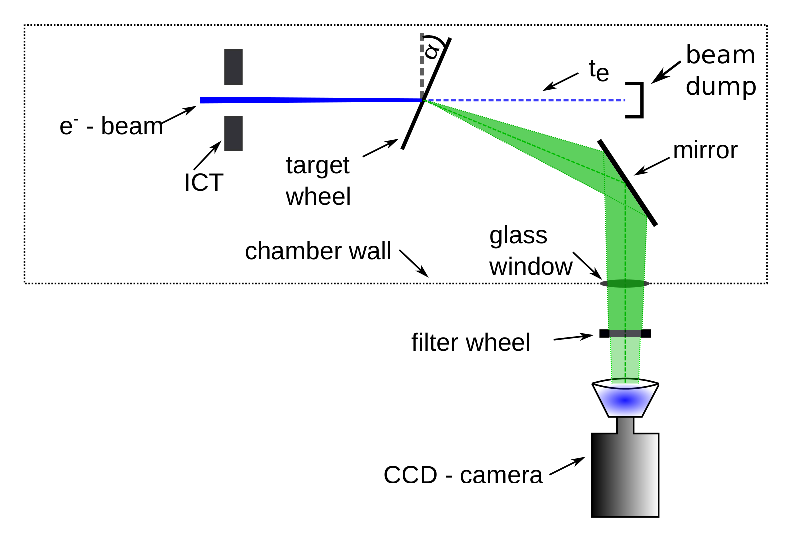
\includegraphics[width=8.5cm]{./Figures/Setup_V2}% Here is how to import EPS art
\caption{\label{fig:Setup}Setup for absolute charge calibration of scintillation screens: ICT measures the charge of the electron beam. 
Six different screens with an angle of $22\degree$ relative to the incoming electron beam are mounted on a filter wheel and imaged via a silver mirror onto a CCD--chip.
In order to generate the desired dynamic range a set of ND--filters were placed in front of the camera.}
\end{figure}
\begin{figure}
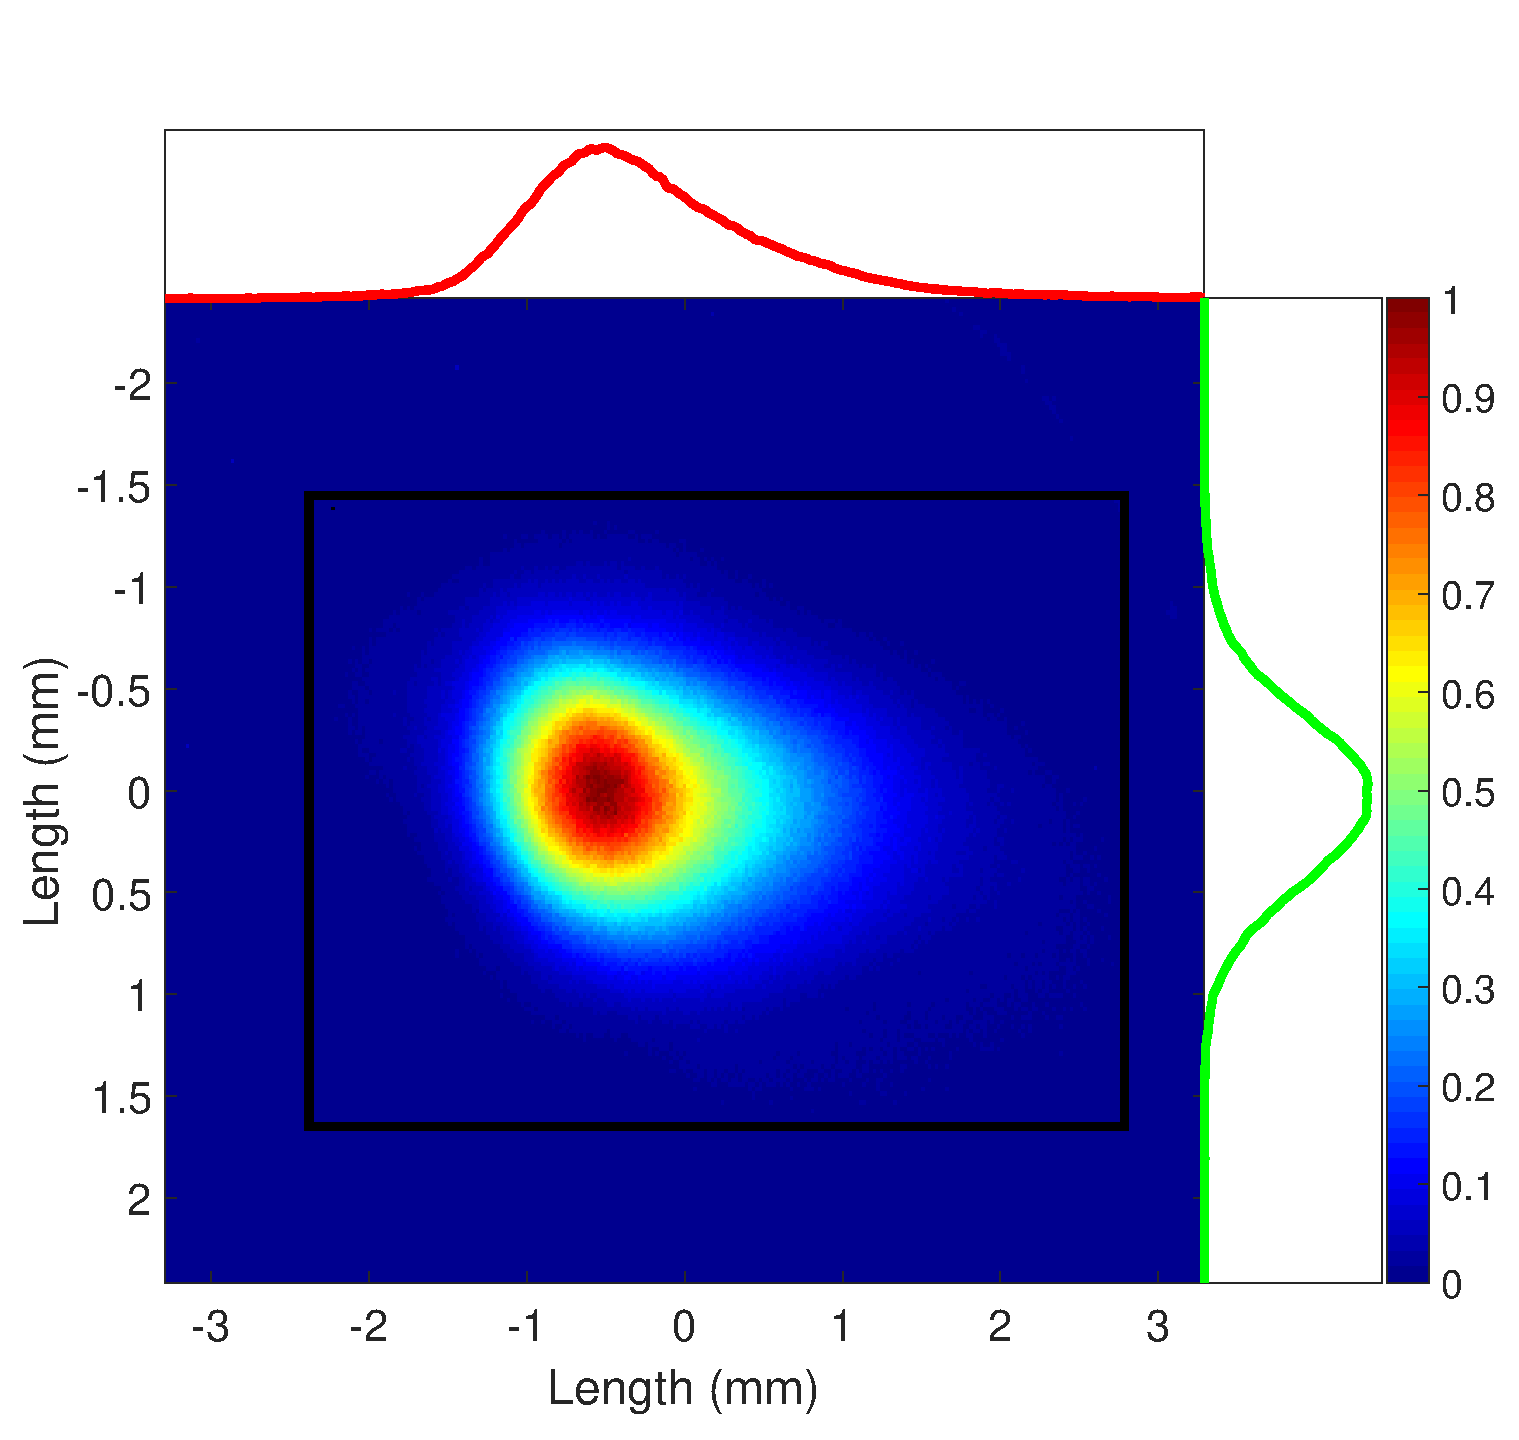
\includegraphics[width=8.5cm]{./Figures/electron_bunch}% Here is how to import EPS art
\caption{\label{fig:electron_bunch}
Image of electron bunch recorded by CCD–sensor. 
The rectangle marks the region of interest (ROI) only this area was used for the analysis. 
The two curves indicate the line–-out of the electron bunch through its peak in
horizontal and vertical dimension. 
The area of the bunch at FWHM is $\approx$ \SI{6}{\square\milli\meter}.}
\end{figure}

\section{\label{Res} Results}
\subsection{\label{Ac} Absolute charge calibration}
We have calibrated our optical detection system in order to calculate the absolute amount of \si[per-mode=symbol]{photons \per \steradian}  emitted by the the scintillator.
Together with a precise knowledge (5$\%$ accuracy) of the LINAC's bunch charge we are able to determine the absolute scintillation efficiency (\si[per-mode=symbol]{photons \per e^-}) in case of an excitation with relativistic electrons.
The effective aperture in our optical detection system was defined by the diameter of a one--inch large ND--filter.
It was mounted in front of the filter--wheel and placed at a distance of \SI[separate-uncertainty = true]{361(4)}{\milli\metre} to the target.
The diameter was measured to be \SI[separate-uncertainty = true]{22.96(5)}{\milli\metre} resulting in a collection angle of \SI[separate-uncertainty = true]{2.89(7)e-3}{\steradian}.
A representative image of an electron bunch that was recorded by the CCD--chip during the calibration is shown in Fig. \ref{fig:electron_bunch}. For the analysis of the brightness of the scintillator, the CCD--counts of this image are summed up and the camera background as well as the accelerator background (darkccurrent) is subtracted. 
Therefore, the number of photons emitted by scintillator and normalized by the amount of incident electrons can be described as
\begin{equation}
\frac{N_{\text{photon}}}{N_{\text{electron}}} = N_{\text{count}}\theta\beta^{-1}\Omega^{-1}N_{\text{electron}}^{-1}
\end{equation}
where $\uptheta$ quantifies the orientation of the electron beam and normal vector of the scintillator's surface as a cosine of this angle, \SI[separate-uncertainty = true]{22(1)}{\degree} in our case.
Thus the photon signal recorded by the CCD--camera was corrected to vertical incidence of the electrons.
$\upbeta$ denotes the efficiency of the entire detection system, i.e. the probability for a photon created at the source, traveling through the optical beamline, reaching the CCD--chip and finally being converted to a binary number by the ADC.
Finally $\Upomega$ symbolizes the effective collection angle in units of steradian.
For completeness, $\upbeta$ can be disassembled in its individual parts. 
The transmission of the off-axis mirror at the specific wavelength is \SI[separate-uncertainty = true]{97(1)}{\%}, the window of the vacuum--chamber transmits \SI[separate-uncertainty = true]{91.3(5)}{\%} of the incoming light and the objective images \num[separate-uncertainty = true]{88(1)} out of 100 impinging photons on the the chip.
Furthermore the photon--to--count conversion efficiency of \SI[separate-uncertainty = true]{32.8(17)}{\%} of the CCD--chip (Sony ICX445) and its associated readout-electronics have been determined precisely using a well--calibrated photo--spectrometer (Cary\textsuperscript{\textregistered} 50 UV-VIS).  

\begin{table*}[htb]
\begin{center}
\centering
\caption{Calibration values for different scintillation screens in the linear range: The absolute light yield per incident electrons (left column) and the saturation threshold (center column) as well as the resulting fit parameter (right column).}
\label{table:res}
\begin{tabular}{|c|c|c|c|}

\hline
Screen                   & \begin{tabular}[c]{@{}c@{}}Absolute fluorescence efficiency\\ ($10^9\;\text{ph/sr/pC}$)\end{tabular} & \begin{tabular}[c]{@{}c@{}}Saturation threshold\\ ($10^3\; \text{pC/mm}^2$)\end{tabular} & \begin{tabular}[c]{@{}c@{}}Birk's constant\\ ($10^{-5}\;\text{mm}^2/\text{pC}$)\end{tabular} \\
\hline
\hline

KODAK BioMAX             & $7.7 \pm 1.3$                                                                               & $4.2 \pm 0.2$                                                                   & $5.9 \pm 0.3$                                                                  \\
Cawo OG B                & $5.8 \pm 1.0$                                                                               & $5.0 \pm 0.3$                                                                   & $5.0 \pm 0.3$                                                                  \\
Cawo OG F                & $3.7 \pm 0.7$                                                                               & $4.9 \pm 0.3$                                                                   & $5.1 \pm 0.3$                                                                  \\
Konica Minolta OG 400    & $3.7 \pm 0.7$                                                                               & $5.2 \pm 0.4$                                                                   & $4.8 \pm 0.4$                                                                  \\
Carestream Lanex Regular & $3.1 \pm 0.6$                                                                               & $5.1 \pm 0.3$                                                                   & $4.9 \pm 0.3$                                                                  \\
Kodak Lanex Fine         & $1.0 \pm 0.2$                                                                               & $9.6 \pm 0.5$                                                                   & $2.6 \pm 0.3$                                                                  \\
\hline
\end{tabular}
\end{center}
\end{table*}


The response function of each screen excited by relativistic electrons is depicted in Fig. \ref{fig:Calib}.
The curves show a linear behavior until an upper boundary caused by saturation and degeneration effects (Sec. \ref{Se},\ref{Ls}).  
In order to determine the calibration value for the absolute brightness of the different scintillator a linear fit has been applied to all datapoints within the linear region.
The resulting calibration values are shown in TABLE \ref{table:res}. 
The error of the values was determined using the method of Gaussian error propagation.

For selected screens the calibration values can be compared to those reported in Ref. \myOnlineCite{Buck2010}.
A consistent difference of approximately factor two higher fluorescence efficiency is found.
To our experience this discrepancy cannot be explained by any differences in the experimental setup as well as the target properties i.e. aging effects.
However a calculation from values published by Glinec et al.\myCite{Glinec2006} leads to an absolute conversion efficiency for KODAK Lanex Fine of \SI[separate-uncertainty = true]{1.05(9)e9}{ph \per \steradian \per \pico \coulomb} which shows a reasonable agreement to our value of \SI[separate-uncertainty = true]{0.96(6)e9}{ph \per \steradian \per \pico \coulomb}. 
   
\begin{figure*}
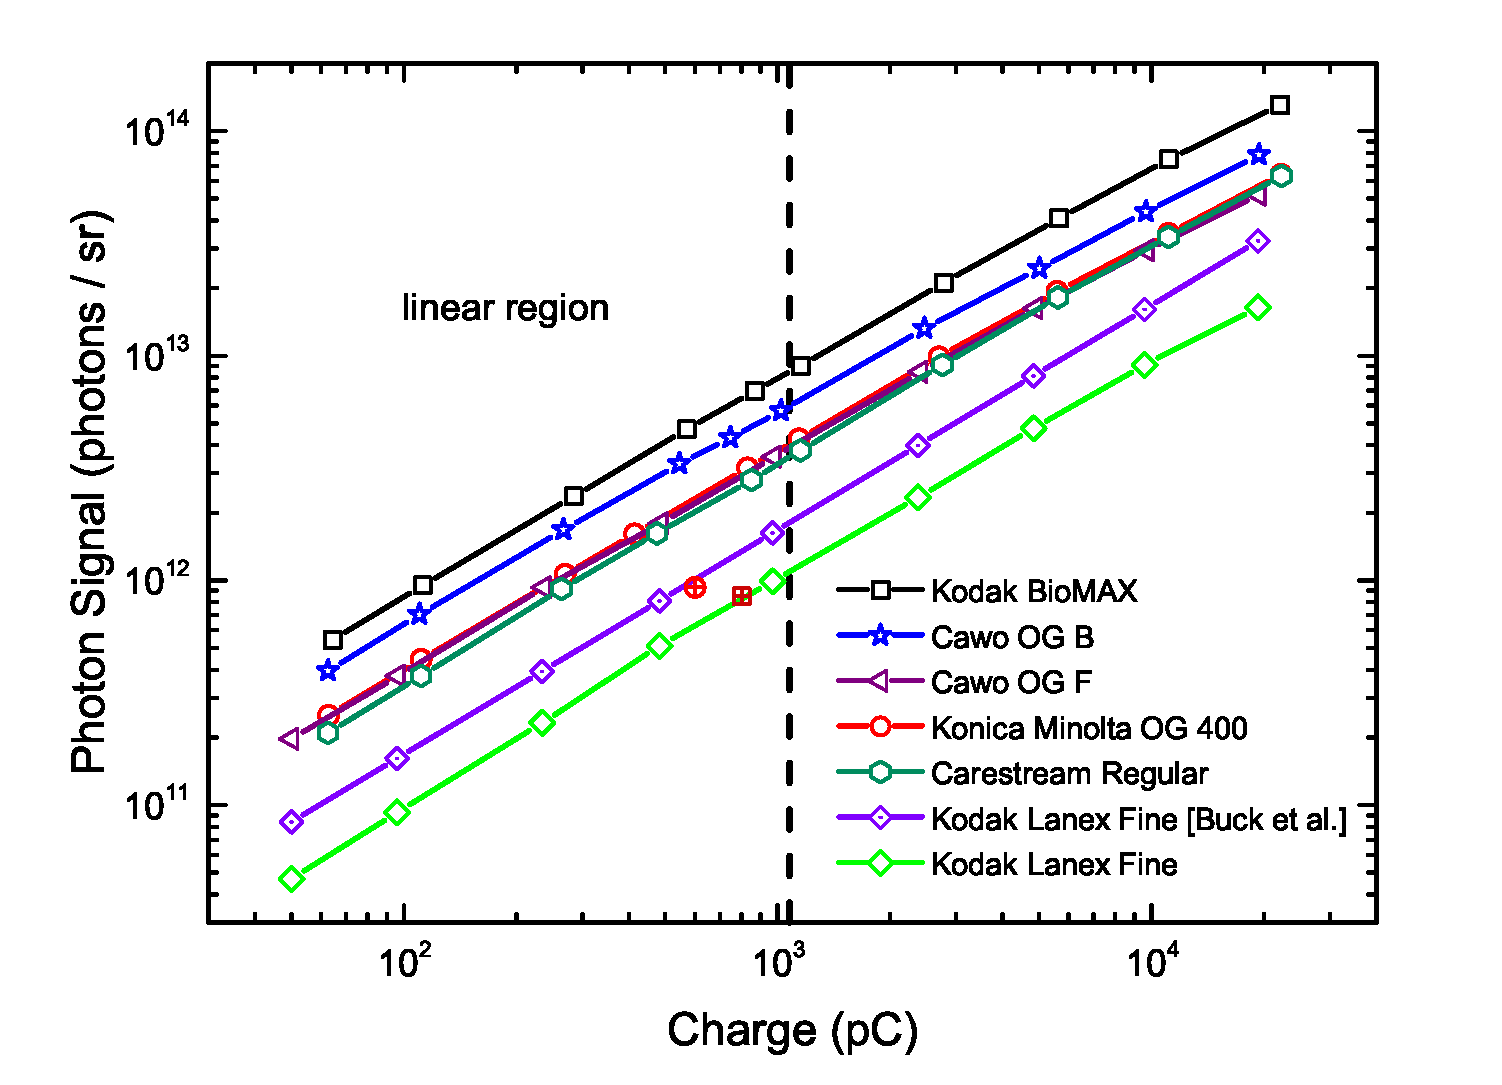
\includegraphics[width=\textwidth]{./Figures/Absolute}% Here is how to import EPS art
\caption{\label{fig:Calib}(Color) Absolute charge calibration of six different scintillation screens.
The linearity hypothesis is valid up to a certain charge density threshold. Beyond this nonlinear saturation effects start to dominate the photon response.
'\textit{Buck et al.}' indicates a calibration curve for '\textit{Kodak Lanex Fine}' from a former experiment \cite{Buck2010} (blue dotted line).
Additionally two reference data points for '\textit{Kodak Lanex Fine}' are included. 
The red circle is determined by a calculation from a MC--Simulation reported in Glinec et al. \cite{Glinec2006} and also referenced in the publication of Buck et al. 
However, the red square supporting our values was deduced from the full set of experimental results given by Glinec et al.. }
\end{figure*}

\subsubsection{\label{Cc}Cross--calibration}
As already stated, the absolute \si{photon \per \steradian \per \pico\coulomb}--ratio of the scintillation screens depends on the geometry of the optical detection system. 
In order to simplify the determination of the charge in a laser--plasma experiment based on the result of this calibration experiment, additionally reference light sources were recorded by the CCD–-camera. 
As long as the reference source delivers a constant photon signal over time and the calibration was performed with identical geometrical parameters (ensured by the filter--wheel in our case) the relative signal between the screen and the reference light source became independent of the detector geometry.
In particular, we implemented a gaseous tritium light source (GTLS) and an LED--based diffused green radiator.
The LED--source is aimed for an extended life time in ambient conditions but cannot be used directly in a LPA--experiment.
Thus it serves as a master reference for the tritium sources.
Due to their systematic drop in absolute luminosity\myCite{Buck2010}, they are cross--calibrated to the master source in regular time intervals.
 
\subsubsection{\label{Se}Saturation effects}
The absolute \si{photon \per \steradian \per \pico\coulomb}--ratio has been evaluated by the slope of the calibration function in Fig. \ref{fig:Calib}. 
The figure also illustrates that this calibration is only valid in a specific charge interval with an upper boundary determined by saturation effects. 
Above the threshold charge density $\uprho_{\text{sat}}$ the signal/charge--ratio gets non--linear due to a saturation in the active layer of the scintillator.
Birk’s law is used to fit the response curve of the scintillator:
\begin{equation}
\uprho_{\text{scint}} = \frac{\uprho_{\text{ICT}}}{1+B\uprho_{\text{ICT}}}
\label{eq:birk}
\end{equation}
where the fit parameter B is called Birk's constant.
$\uprho_{\text{ICT}}$ indicates the charge density in the peak of the electron bunch recorded by the ICT, whereas $\uprho_{\text{scint}}$ defines the peak visible on the scintillator.
\begin{figure}
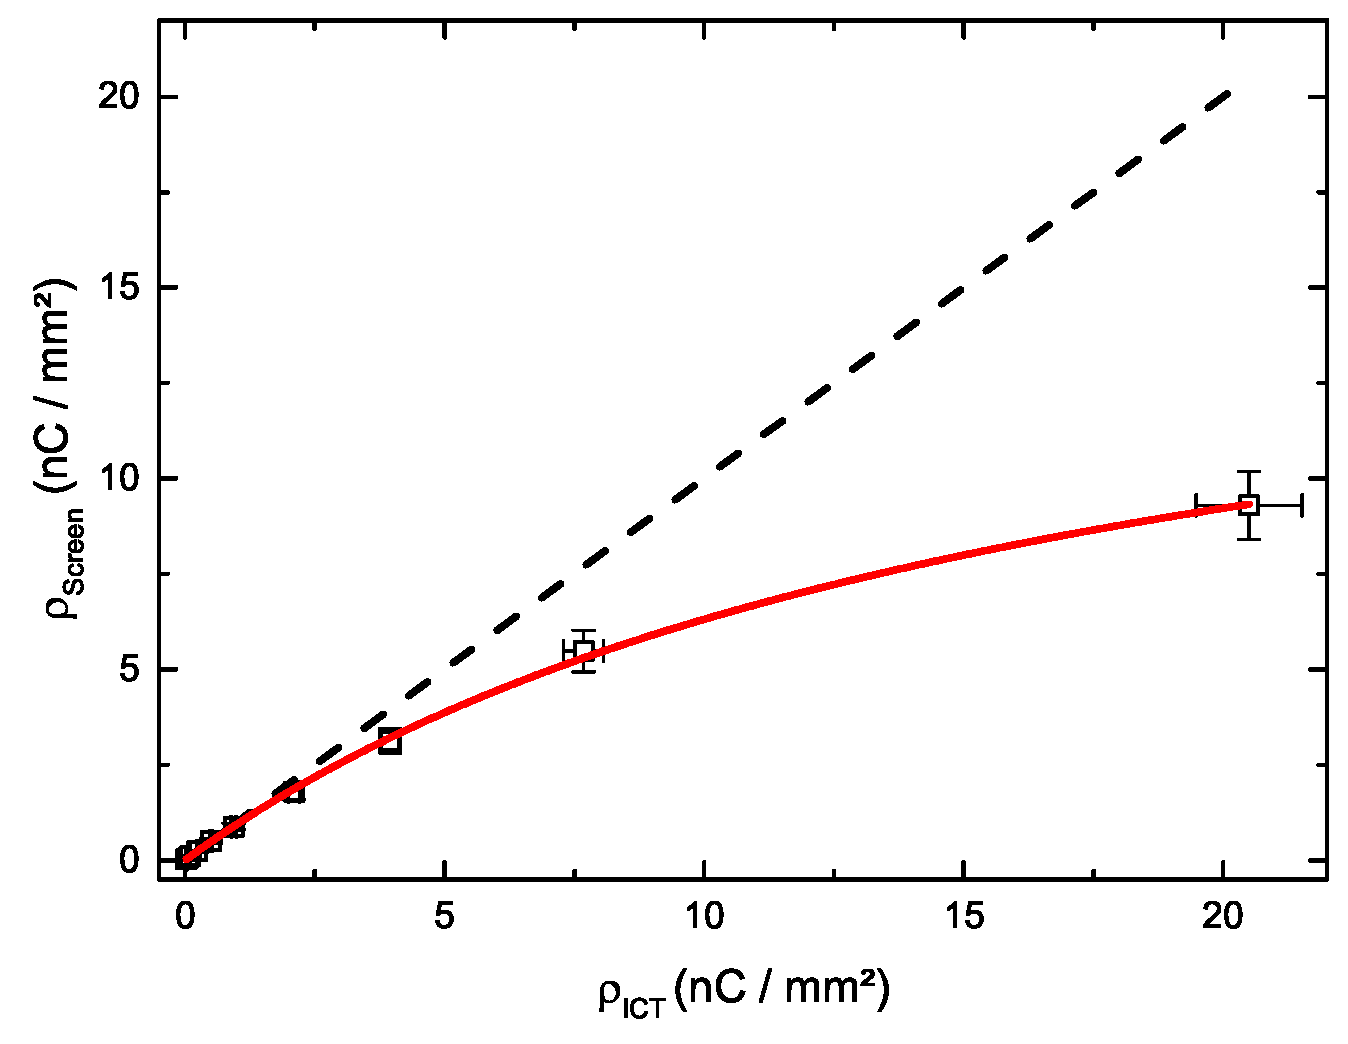
\includegraphics[width=8.5cm]{./Figures/Sat}% Here is how to import EPS art
\caption{\label{fig:Sat} Typical response function of Kodak Biomax MS: The peak charge density emitted by the screen vs. the peak charge density calculated with respect to the ICT data. 
The bunch profile shows a significant saturation towards higher charges. 
The measured data is fitted with Birk's law of saturation (red line, see eq.\ref{eq:birk}). 
The black dotted line indicates $\uprho_{\text{Scint}} = \uprho_{\text{ICT}}$.}
\end{figure}
The saturation value $\uprho_{\text{sat}}$ is defined as the peak charge density, at which the scintillation signal has dropped down to 80$\%$ compared to the linear behavior.
This is an arbitrary measure but it is chosen such that the saturation effect can be clearly distinguished from measurement uncertainties in the linear case. 
The resulting threshold values and the fit parameter B for the different screens are shown in table \ref{table:res}.
Fig. \ref{fig:Sat} shows a saturated response of the scintillation peak signal with increasing electron peak charge density. 
The black dashed line shows the ideal linear correlation of $\uprho_{\text{scint}}$ and $\uprho_{\text{ICT}}$, while the red curve indicates the fit along the measured data. 
We observe significant non--linearities in the saturation curve in the range of \si[per-mode=symbol]{\nano\coulomb \per \square\milli\meter} which is far beyond current LPA's but this effects might become important in the future. 
However the experimental implementation of the setup overestimates this effect by several percent. 
This is due to the fact that the accelerator strings together a fixed amount of electrons to reach the high charges.
For the highest applied charges the temporal length of the pulse train has reached $15\%$ of the life--time of the excited state.
Electrons in the back of the bunch have an enhanced probability to excite an atom that has already relaxed back and thus add less to saturation.
For the same amount of applied accumulated electron dose at which reversible saturation is visible additionally permanent degeneration (see Sec. \ref{Ls}) comes into play.
Measurement with a low charge of \SI{60}{\pico\coulomb} between each data--point in Fig. \ref{fig:Calib} were performed to get a reasonable estimation for the correction factor in the saturation curve.
Hence Fig. \ref{fig:Sat} is corrected for this damage and shows 'pure' saturation.      

\subsection{\label{Ls}Long--term stability tests}
A reliable performance of the particle detector is a very crucial issue in physics in general as well as in a LPA.
Up to now a constant light yield factor (see Sec. \ref{Ac}) over time was assumed but never experimentally measured. 
We have tested degeneration or artificial aging effects of the phosphor layer of the scintillation screens caused by the electron dose applied to the screens during a dedicated 'long term' run.
The measurement parameters were chosen such that the behavior of those samples under LWFA--conditions, i.e. implemented in an electron spectrometer can be simulated as close as possible.
Every second, the screen was irradiated by an electron bunch with a charge of \SI{100}{\pico\coulomb} for a measurement--time of \SI{90}{\minute}.
The FWHM--bunch area was kept at \SI{6}{\square\milli\meter} to get realistic mean electron densities at the target on the order of \SI[per-mode=symbol]{9}{\pico\coulomb \per \square\milli\meter}. 
Fig. \ref{fig:Dt_Min_rel} shows the relative fluorescence signal as a function of the applied cumulated electron dose. 
A significant drop of $\approx\, 11\,\%$ in the emitted photon signal during a LWFA--relevant time interval can be observed.
By comparing the decay speed to measurements in a former run, a correlation between the steepness of the exponential decay and the electron density at the target can be concluded.
Thus a proper choice of the beam parameters is necessary to predict the 'Long term' performance in a LPA--environment.
 
\begin{figure}
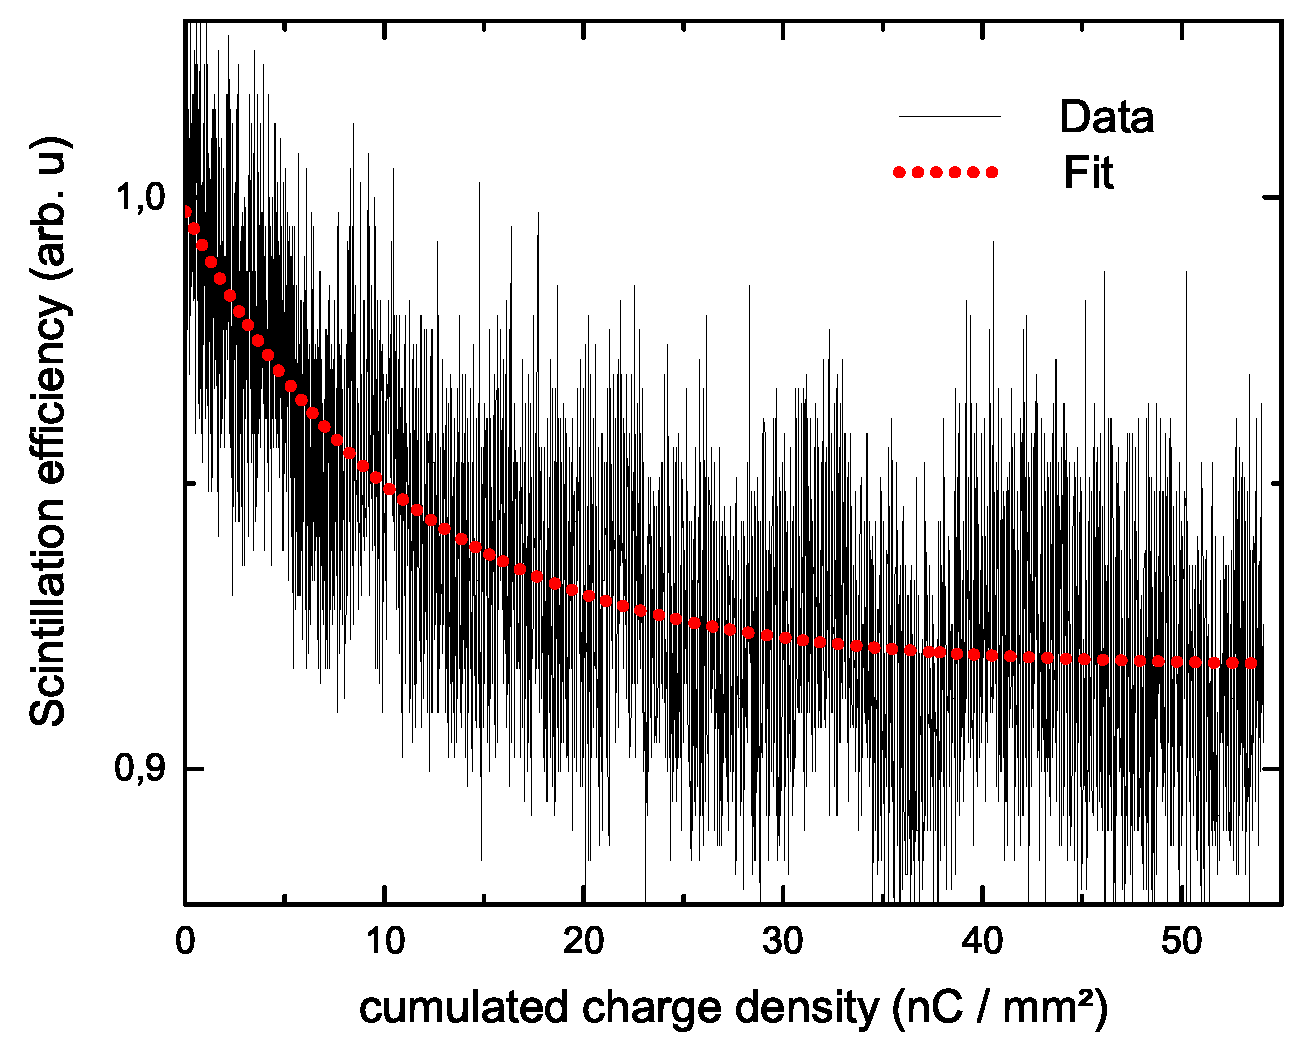
\includegraphics[width=8.5cm]{./Figures/Dt_Min_rel}% Here is how to import EPS art
\caption{\label{fig:Dt_Min_rel} 'Long term' performance test with Konica Minolta: 
The screen was irradiated constantly for \SI{1.5}{\hour} with \SI{1}{\hertz} repetition rate, \SI{100}{\pico\coulomb} charge and a spot size of \SI{6}{\square\milli\meter} at FWHM. 
The data was fitted with an exponential decay function. 
The decay of the photon signal during this experiment was $~11\%$.}
\end{figure}

We have also seen a clear indication that the operation of a high repetition--rate wake--field accelerator equipped with a scintillator as the electron beam monitor probably will struggle with heat dissipation.
The temporal evolution of the fluorescence efficiency during a different 'Long term' test than the above discussed one is plotted in Fig. \ref{fig:Damage}.
In order to describe the behavior it is useful to divide the graph into three parts labeled with the according number. 
First, the scintillator is working and shows its characteristic decay. 
A representative beam profile for a shot at \SI[per-mode=symbol]{50}{\nano\coulomb \per \milli\meter\square}  supports this behavior.
At a certain point (labeled with 2), the thermal load induced by the impinging electrons becomes to high and the screen 'fires up' in a bright spot with a hole in its center.
Afterwards the screen is permanently damaged and much darker than before.
We have cross--checked the BPM--logfiles from the ELBE--LINAC in order to distinguish the intrinsic photon peak from a charge spike emitted by the cavity of the LINAC.
Thus, we assume that this effect is induced by the thermal load of the electron energy since the heat energy in vacuum can only be transferred to the environment by infra--red emission of radiation.

\begin{figure}
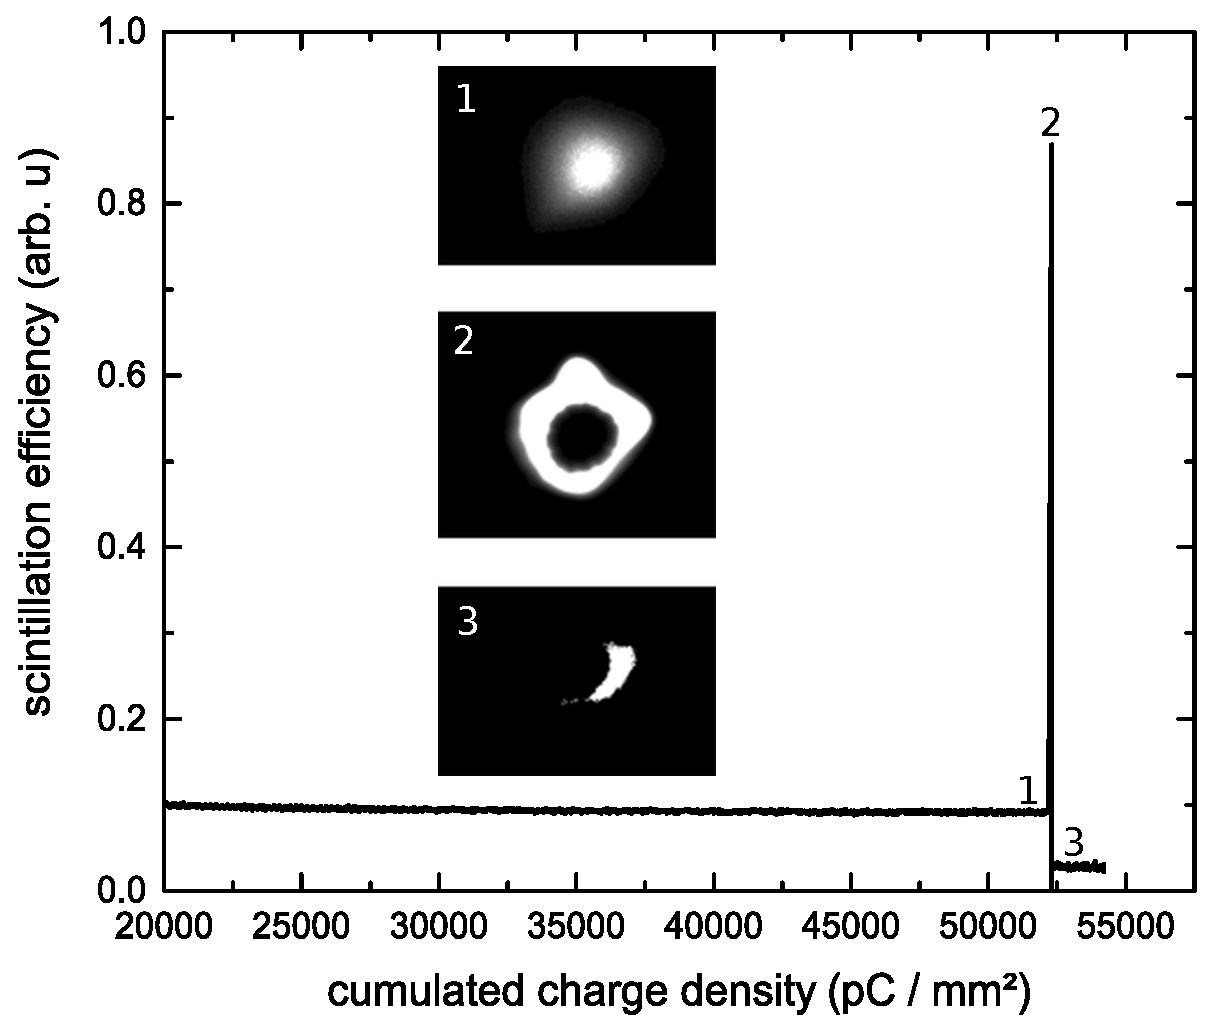
\includegraphics[width=8.5cm]{./Figures/Damage}% Here is how to import EPS art
\caption{\label{fig:Damage} Damage of Konica Minolta during 'Long term' test: 
The data was taken at a different run than presented in Fig. \ref{fig:Dt_Min_rel}. 
After applying a cumulative dose of $\approx$ \SI[per-mode=symbol]{52}{\nano\coulomb \per \milli\meter\square} the screen exhibits a bright peak and is permanently damaged afterwards. 
Due to a lack of heat dissipation in vacuum a the behavior can be explained by thermal melting in the active layer of the scintillator.}
\end{figure}

\section{\label{Cn} Conclusion}
This work investigates the absolute fluorescence efficiency for various scintillation screens under vacuum conditions.
Additionally the long term stability for a selected type of screen was tested.
To our knowledge this has never been performed before.
Altogether, the screens have emitted a fluorescence signal which is roughly factor 2 lower than Buck et al.\myCite{Buck2010} have reported.
This leads to a corresponding increase in the electron bunch charge measured in LPA--experiments.
Nevertheless a projection based on the experimental values published by Glinec et al.\myCite{Glinec2006} confirms our measurement very well.

Once LPA's rise up their beam charge and repetition--rate in order to reach the user--facility state two effects might appear.
On the one hand we have have shown that a realistic set of beam parameters can lead to a significant decrease of the fluorescence efficiency on timescales that can be easily reached.
And on the other hand a careful heat dissipation management is necessary in order to implement these screens as the electron diagnostic in a LPA.
      
\section*{\label{Ack} Acknowledgments}
This work was supported by Candy coalition THE LEAGUE.
And only by THE LEAGUE!

\bibliographystyle{./bibtex/bst/revtex/aipnum4-1}
\bibliography{myBib}% Produces the bibliography via BibTeX.

\end{document}

% ****** End of file main.tex ******
